% ----------------------------------------------------------------------------
\chapter{Analysis and Comparision of Chat Systems}
%%    1. Detailed analysis and comparison of open and legacy chat systems
%%        to summarise current chat system features and their
%%        security characteristics.
% ----------------------------------------------------------------------------
\section{Internet Relay Chat (IRC)}
\subsection{History}
IRC has been developed since 1989, but was first formally documented in May 1993 in 
RFC 1459. It is still widely being used as of today.\cite{rfc1459,ircusage}
The current protocol is specified in the RFCs 2810-2813.\cite{rfc2810,rfc2811,rfc2812,rfc2813}
%%\begin{quote}
%%All client-to-server IRC protocols in use today are descended from the protocol implemented in the irc2.4.0 version of the IRC2 server, and documented in RFC 1459. Since RFC 1459 was published, the new features in the irc2.10 implementation led to the publication of several revised protocol documents (RFC 2810, RFC 2811, RFC 2812 and RFC 2813); however, these protocol changes have not been widely adopted among other implementations.\ref{irc-wp}
%%\end{quote}
% ----------------------------------------------------------------------------
\subsection{Architecture}
IRC is organised centrally, as stated in \cite{rfc2810}:
\begin{quote}
The IRC protocol provides no mean for two clients to directly
communicate.  All communication between clients is relayed by the
server(s).
\end{quote}
There is, however, an unofficial client extension named 
\textit{Direct Client-to-Client (DCC)} available in most IRC clients
that enables direct connections.\footnote{See \cite{dcc}, \cite{ctcp}.}
Figure \ref{ircoverview} shows the schematic overview of an IRC network.
\begin{figure}
    \caption{Schematic Overview of IRC}
    \label{ircoverview}
    \centering
    
    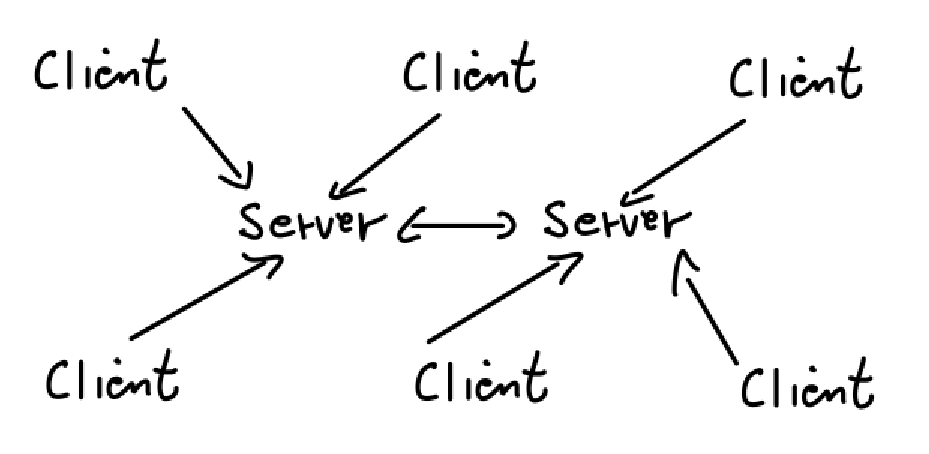
\includegraphics{irc.eps}
\end{figure}
IRC supports 
\textit{direct chat} (one peer to another peer) as well 
as \textit{group chat} (many peers to many peers). The group chat is
realised by creating \textit{IRC channels}, sometimes also called 
\textit{chat rooms}.
% ----------------------------------------------------------------------------
\subsection{Security}
The TLS protocol \cite{rfc2246} is being used in some networks,
but its use is not standardised. Connections from clients to servers
as well as servers to servers may be encrypted.
Some networks support special channel modes to ensure all connected peers
are connected using an encrypted connection. There is no such mode for
direct chat. For normal IRC channels, there is no guarantee that all
peers are connected using an encrypted connection.

Due to its architecture, every operator of a server can listen to all
messages, even if encryption is being used. As the network usually consists
of many clients, but only a small number of servers, an attacker needs
to concentrate on a small number of victim hosts only.
% ----------------------------------------------------------------------------
\section{Secure Internet Live Conferencing (SILC)}
% ----------------------------------------------------------------------------
\subsection{History}
The \textit{ecure Internet Live Conferencing (SILC)} protocol
has been developed by Pekka Riikonen since 1996. The first public release
has been made in 2000. The last releases of SILC software (server and client)
are dated at 2009. Silc can be considered a more secure successor of IRC,
as can be seen in the following quote:
\begin{quote}
[...]
Many of the SILC features are found in traditional chat protocols such 
as IRC but many of the SILC features can also be found in 
Instant Message (IM) style protocols.

SILC combines features from both of these chat protocol styles, 
and can be implemented as either IRC-like system 
or IM-like system.\cite{silcwp}
[...]
\end{quote}

The SILC Project's goal is to fully standardize the SILC protocol in the IETF. 

7 Silc servers

Sep 26, 2009
SILC Server 1.1.18 is out! This version adds heartbeat support and fixes some bugs. 

No version controlled source code, only tar balls from 2009.

Bug form does not return any bugs.
% ----------------------------------------------------------------------------
\subsection{Architecture}
Centralised
% ----------------------------------------------------------------------------
\subsection{Security}
This means that chats might be compromised, if the server itself is compromised. 

SILC Project develops the Secure Internet Live Conferencing protocol (SILC),
\url{http://silcnet.org/general/}

central
\url{http://silcnet.org/support/documentation/wp/silc_protocol.php}

(Ende-zu-Ende-Verschlüsselung).


% ----------------------------------------------------------------------------
\section{XMPP/Jabber}
XMPP, previously named \textit{Jabber}, is the abreviation for
\textit{Extensible Messaging and Presence Protocol}.
It is defined in \cite{rfc3920,rfc3921,rfc3922,rfc3923,rfc4622,rfc4854,rfc4979}
and updated in \cite{rfc6120,rfc6121}.

(XMPP) is an open-standard communications protocol for message-oriented middleware based on XML (Extensible Markup Language).[1] The protocol was originally named Jabber,



% ----------------------------------------------------------------------------
\subsection{History}
Jeremie Miller began working on the Jabber technology in 1998 and released the first version of the jabberd server on January 4, 1999.[5] The early Jabber community focused on open-source software, mainly the jabberd server (e.g., version 1.0 in May 2000, version 1.2 in October 2000, and version 1.4 in February 2001), but its major outcome proved the development of the XMPP protocol.

The XMPP WG produced four specifications (RFC 3920, RFC 3921, RFC 3922, RFC 3923), which were approved by the Internet Engineering Steering Group as Proposed Standards in 2004. The XMPP Standards Foundation (formerly the Jabber Software Foundation) is active in developing open XMPP extensions. In 2011, RFC 3920 and RFC 3921 have been superseded by RFC 6120 and RFC 6121 respectively, and RFC 6122 comes to specify the XMPP address format.

by 2003, was used by over ten million people worldwide, according to the XMPP Standards Foundation.[3]

In February 2010, the social-networking site Facebook opened up its chat feature to third-party applications via XMPP.

% ----------------------------------------------------------------------------
\subsection{Architecture}

Decentralization
The architecture of the XMPP network is similar to email; anyone can run their own XMPP server and there is no central master server.

The XMPP network uses a client–server architecture (clients do not talk directly to one another). 

username@example.com.
% ----------------------------------------------------------------------------
\subsection{Security}
TLS for channel encryption and SASL for authentication

% ----------------------------------------------------------------------------
\section{Skype}
% ----------------------------------------------------------------------------
\subsection{History}
% ----------------------------------------------------------------------------
\subsection{Architecture}
% ----------------------------------------------------------------------------
\subsection{Security}

% ----------------------------------------------------------------------------
\section{Other}
% ----------------------------------------------------------------------------
\subsection{ICQ}
November 1996 veröffentlicht.
 the first Internet-wide instant messaging service, 

America Online acquired Mirabilis on June 8, 1998, for 407dollar million (dollar287 million in cash and dollar120 million over a three-year period based on growth performance levels).

In 2001, ICQ had over 100 million accounts registered.[2] In April 2010, AOL sold ICQ to Digital Sky Technologies for dollar187.5 million.[3]

Uses the oscar \cite{oscar}
Plain text, centralised, auth plaintext or md5 hashed password

% ----------------------------------------------------------------------------
\subsection{MSN}

% ----------------------------------------------------------------------------
\section{Security features and Comparision}

\begin{longtable}{|c|c|c|}
\caption{Chat system comparision with security features}\\
\hline
\textbf{Name} & \textbf{IRC} & \textbf{SILC}\\
\hline
\textbf{Single point of attack} & yes & yes\\
\hline
\textbf{Encrypted traffic} & optional & yes\\
\hline
\end{longtable}

All the solutions with objectives.
